% RQ1
\section{Empirical study}
\label{sec:empiricalstudy}
% Both state of the art tools
% But also commonly used simpler tools
This section will be dedicated to the methodology to answer the first research question: \textit{What is the current state of the art and what is the performance of these tools?}; 

The first part of the research question is covered by \autoref{chap:selectedtools}. Those tools are selected to represent the state of the art of error detection tools.
To answer the latter part of the question and substantiate further research questions with research data, an empirical study on error detection tools and different configurations is designed. To cover a broad range of configurations (strategies) of these tools, a range of permutations of configurations will be generated for each error detection tool and run on a wide range of datasets with different characteristics and errors. The source code of this framework can be found on GitHub\footnote{\url{\githubsource}}.
~\\Because the source languages of error detection tools differ, a high-level general purpose programming language suits to be used for the framework to connect all the different underlying tools. Together with the fact that it has well-supported libraries for relational data handling, Python\footnote{\url{\pythonsource}} was chosen as the main development language.


\subsection{Setup}
\label{subsec:setup}
First, the setup for the empirical study will be discussed. The basic setup is shown in \autoref{fig:empiricalsetup}. For each tool in the study, a number of configurations is created, depending on the configurability of the tool. Each configuration in combination with that tool, will be tested on all the available datasets. So a single experiment exists of:
\begin{itemize}
    \item An error detection tool
    \item A tool specific configuration
    \item A target dataset
\end{itemize}

Each experiment will be pushed to the queue of experiments, allowing for retrieving a experiment session without having to rerun all the finished experiments. Incrementally, all the experiment results are pushed into the results database, allowing for the empirical study and further usage with performance prediction and tool ranking. 

\begin{figure}[h]
    \centering
    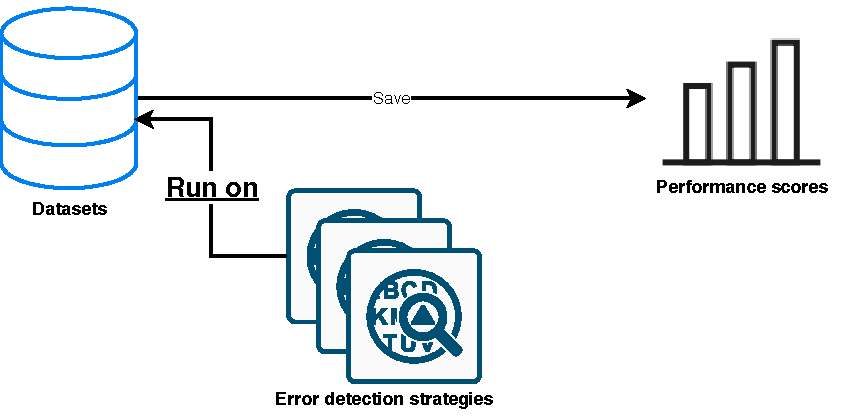
\includegraphics[width=0.9\textwidth]{thesis/Figures/Method/PerformanceEstimation-Experiment.pdf}
    \caption{Setup of the empirical study}
    \label{fig:empiricalsetup}
\end{figure}

% Error detection API to do experiments
\subsection{Error detection framework}
A framework for running error detection tools was designed. The purpose of creating a single framework is to have homogeneous in and output for each selected error detection strategies, creating the possibility of running batches of experiments in a structured manner. 
The content and structure of the error detection framework is as follows:
\begin{itemize}[label=\ding{212}]
\item dataset
\item experiment
% \item helpers
%     \begin{itemize}[label=\ding{212}]
%         \item autofd
%         \item autoregex
%     \end{itemize}
\item profiler
\item tool
\item tools (see \autoref{chap:selectedtools})
\end{itemize}

\paragraph{dataset} contains the class for handling datasets for the experiments. It is based upon the work done by \cite{Mahdavi2019-zf} where each dirty dataset has a clean counterpart. Errors can be calculated both cell-wise as well as row-wise. Information about a dataset can be uploaded for later use and metrics like precision, recall and the F1-measure can be calculated from within this class.

\paragraph{experiment} contains the workflow depicted in \autoref{fig:empiricalsetup}. Objects from this class can create the tool-configuration-dataset triples for the empirical study. Also, it contains the incremental queuing system for execution of experiments, which can be interrupted and resumed at will. Besides the workings shown in \autoref{fig:empiricalsetup}, this part of the framework supports timeouts of the experiments, to shut down experiments whenever the preconfigured time limit is set. Lastly, it will upload the result metrics, configuration and runtime to a centralized database to further filter and analyze the results.

\paragraph{profiler} contains the elements to profile datasets and predict performance for different tools. This will be further discussed in \autoref{sec:performanceprediction}.

\paragraph{tool} contains the classes for creating error detection tool instances and the base class for tool. The tool creator dynamically finds added tools and is possible to return "Tool" instances for each error detection tool. Each error detection tool is adjusted to work in similar fashion. The tool base class contains an abstract method to run the code, expecting similar input and output for each tool. The tool base class has subprocess functionality to support the timeouts set by the experiment and to run non-Python code. The tool base class also cleans up left over subprocesses whenever timeouts are reached. 

\paragraph{tools} contains each error detection specific implementation of the Tool base class. Only the initialization and the \verb|run| method need to be implemented for each tool work, making it easy to extend this framework. Every tool is implemented in a different submodule. The implemented tools are discussed in \autoref{chap:selectedtools}.

\subsection{Datasets}
\label{subsec:datasets}
The datasets selected contained different types of errors, to create a heterogeneous test set to compare the tools and configurations. Errors in a dataset are defined by the difference in the dirty dataset and clean dataset. So only the ground truth makes up an error. Errors can be seen as a transformation of the ground truth to some dirty value. These transformations could specify why the dirty version is wrong. Below are different "error types" that describe errors that have similar transformation between the dirty instance and the ground truth. Of course, there might be overlap in these transformation, as one type of transformation could have the same effect as another type, but these categorizations give an overview of the dataset quality one has to deal with.

\subsubsection{Error types}
The error types are derived from \autoref{subsec:errortypes}, with the addition of the "other errors", which contains errors that cannot be found or described by the default error type categories. These are summaries and common examples of the main error types:

\begin{itemize}
    \item \textit{Outliers:} Values that are erroneous and do not fit in the (column) distribution of the dataset
    \item \textit{Pattern violations:} Values that are erroneous and do not fit in the common pattern of that column (i.e. 2k20 in stead of 2020). Also error values that contain wrong spelling belong to this category.
    \item \textit{Rule violations:} This category contain the violations of dependencies and/or more complex rules between columns. Also empty values or missing value placeholders (e.g. N/A) belong to this category. Lastly, inconsistent abbreviations or references to entities (like states, companies, universities, etc..) also count as rule violations.
    .\item \textit{Duplicates:} These errors are different tuples, referring to the same real-world entity, while only one reference should be valid.
    \item \textit{Other error types:} Examples of this type are values that are result of a classification (output) based on the other given columns, but the output is wrong. An error value where the content of the entity is erroneous, but other rules and patterns do hold. 
\end{itemize}

\subsection{Execution \& Evaluation}
To answer the last part of research question 1; \textit{What is the current state of the art and what is the \textbf{performance of these tools?}}; different parts from the sections above will be combined. The tools from \autoref{chap:selectedtools} will be run in selected configurations (tool specific) on a variety of the datasets (\autoref{sec:selected_datasets}). Different performance score metrics will be kept for each experiment. In a single experiment, a timeout limit is set to filter out tool configuration that do not satisfy runtime needs. The main performance scores that will be kept are:
\begin{itemize}
    \item Precision
    \item Recall
    \item F1-score
\end{itemize}

The performance scores (results from experiments depicted in \autoref{fig:empiricalsetup}) will be \textbf{aggregated into a table} showing the best results for a \textit{single tool} (regardless of its configuration) and the \textit{target dataset}, sorted on the F1-score. In the table, the rows represent a single dataset, and each column represents a tool. Such a table will allow comparison to see which of the tools performs best for which dataset. This result will show the performance of tools over a wide variety of datasets, holistically for every error type.
Secondly, for each error type (excluding "other error types") as shown in the previous section, separate results will be shown. Instead of tackling the error detection task holistically, experiment results will be shown only for \textbf{overlapping error types} occurring in the dataset and that are presumably detectable by the error detection tool (for error type coverage, see \autoref{tab:tools-error-types}).
Combining the findings from the overall analysis and analysis per error type will give a complete overview of the performance of the selected tools representing the state of the art error detection methods. 

% \\Additionaly, these tables can be repeatedly be created with filters (such as no human interaction) or grouping the best scores per tool and dataset based on the selected metrics (i.e. best precision or best F1-score).